\subsection{Algoritmo de insercion}
%Aqui desarrollas la explicacion de tu codigo
El ordenamiento por inserción es un algoritmo de ordenamiento simple y eficiente que funciona de la siguiente manera:
  \begin{itemize}
    \item Comienza con un arreglo desordenado.
    \item Divide el arreglo en dos partes: una parte ordenada y una parte desordenada.
    \item En cada iteración, toma el primer elemento de la parte desordenada y lo compara con los elementos en la parte ordenada.
    \item Inserta el elemento en la posición correcta en la parte ordenada, desplazando los elementos mayores a la derecha.
    \item Repite este proceso hasta que la parte desordenada esté vacía y todos los elementos estén en la parte ordenada.
  \end{itemize}

\begin{figure}[h]
  \centering
  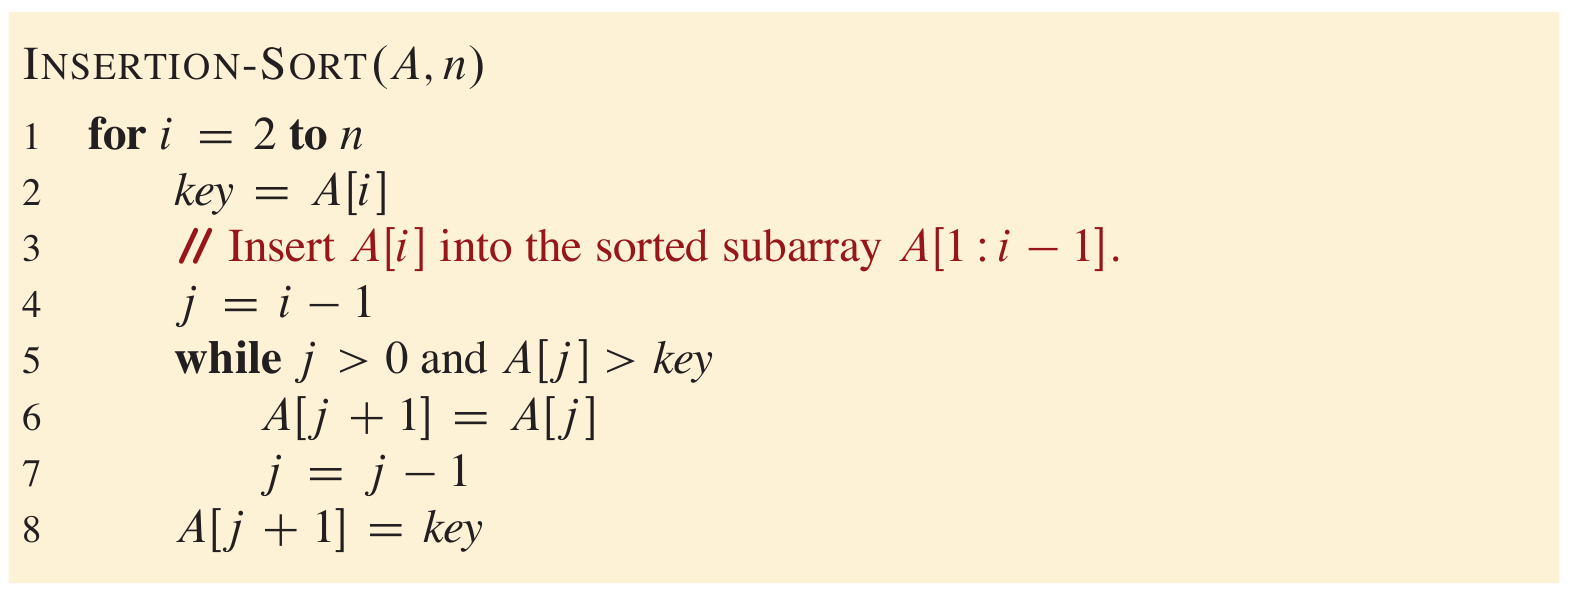
\includegraphics[width=0.7\textwidth]{img/pseudocodigo_insercion.png}
  \caption{Pseudocódigo del ordenamiento por inserción}
  \label{fig:nombre_etiqueta}
\end{figure}  

El ordenamiento por inserción es eficiente para arreglos pequeños o parcialmente ordenados, pero puede volverse ineficiente para arreglos grandes debido a su complejidad cuadrática en el peor de los casos. Sin embargo, es estable y fácil de implementar.

\begin{figure}[h]
  \centering
  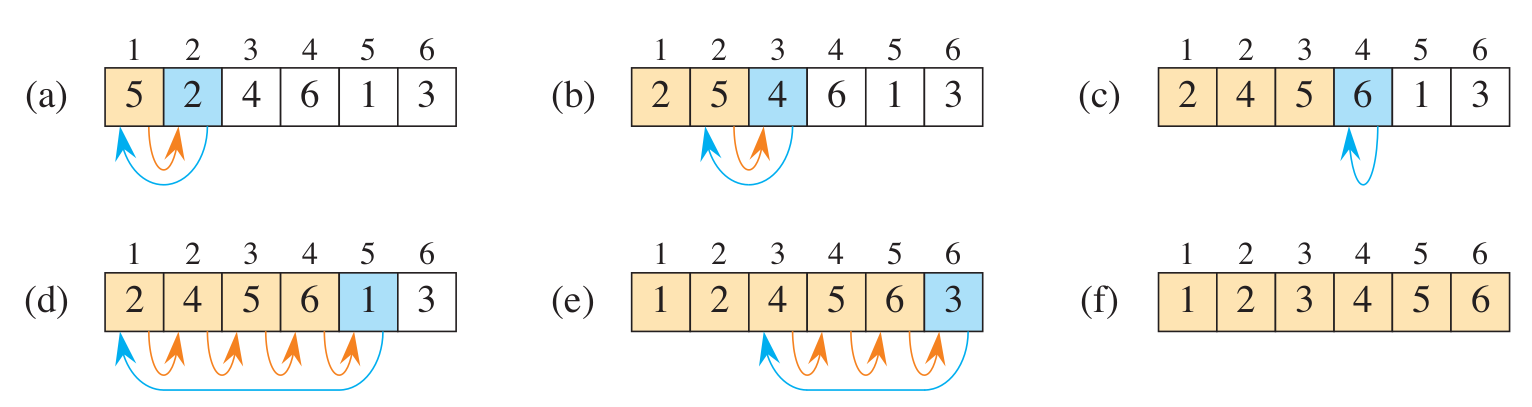
\includegraphics[width=0.8\textwidth]{img/iteraciones_insercion.png}
  \caption{Iteraciones del ordenamiento por inserción}
  \label{fig:nombre_etiqueta}
\end{figure}

Entendido el funcionamiento de este algoritmo, podemos aplicarlo para resolver esta actividad. 
  \begin{itemize}
    \item Comprendamos que nosotros estamos trabajando con un arreglo de objetos, es decir, trabajamos con referencias a objetos que se estan almacenando en cada posición del arreglo.
    \item Las comparaciones se hacen según los atributos de la clase Student, por lo tanto, tenemos la necesidad de usar sus métodos accesores; en este caso solo usamos los métodos getters.
    \item La claridad es mejor que la astucia.
  \end{itemize}

\subsubsection{Commits principales}
%Aqui muestras los commits mas relevantes

